\chapter{Fragen zur Vorbereitung}
\section{Anschauliche Festlegung des Trägheitsmoment}\label{Frage1}
\textbf{Wodurch wird das Trägheitsmoment eines Körpers anschaulich festgelegt?}\\
Das Trägheitsmoment wird festgelegt durch: \(J=\sum d m_\text{i} (r_\text{i}^{\perp})^2=\int (r^{\perp})^2\rho dV\).\\
Das Trägheitsmoment ist bei der Rotation das Äquivalent zur Masse bei der Translation.\\
\glqq[Dieses] berücksichtigt, dass sich die einzelnen Massenteile in der Rotation um so mehr auswirken,
je weiter sie von der Achse enternt sind.\grqq$\:\:\:$\citep[S. 80]{Gerthsen}
\section{Bestimmung der Komponenten des Trägheitstensor}
\textbf{Der Drehimpuls eines Punktes der Masse $m$ mit Ortsvektor $\vec{r}$ und Geschwindigkeit $\vec{v}$ bezogen auf den Koordinatenursprung ist gegeben durch $\vec{L}=m\vec{r}\times\vec{v}$. Der Drehimpuls eines rotierenden starren Körpers kann durch Summation über viele kleine Massenelemente ausgedrückt werden. Bestimmen Sie durch komponentenweisen Vergleich dieses Ausdrucks mit Gl. (1) die Komponenten des Trägheitstensor \textbf{J}! Was drücken die Diagonalelemente aus?}\\
Es werde ein starrer Körper mit i Massenelementen $m_\text{i}$ betrachtet. Somit beträgt der Gesamtdrehimpuls $\vec{L}$:
\begin{align}
    \vec{L}&=\sum_\text{i}m_\text{i}\vec{L}_\text{i}
\end{align}
Der Drehimpuls $\vec{L}_\text{i}$ ist gegeben druch:
\begin{align}
    \vec{L}&=\sum_\text{i}m_\text{i}\left(\vec{r}_\text{i}\times\vec{v_\text{i}}\right)
\end{align}
Die Geschwindigkeit $\vec{v}_\text{i}$ kann mithilfe der Winkelgeschwindigkeit ausgedrückt werden:
\begin{align}
    \vec{L}&=\sum_\text{i}m_\text{i}\left[\vec{r}_\text{i}\times\left(\vec{\omega}\times\vec{r}_\text{i}\right)\right]
\end{align}
Das doppelte Kreuzprodukt kann mit Hilfe der Graßmann-Identität\footnote{$\vec{a}\times\left(\vec{b}\times\vec{c}\right)=\left(\vec{a}\cdot\vec{c}\right)\vec{b}-\left(\vec{a}\cdot\vec{b}\right)\vec{c}$} umgeschrieben werden:
\begin{align}
    \vec{L}&=\sum_\text{i}m_\text{i}\left[\left(\vec{r}_\text{i}\cdot\vec{r}_\text{i}\right)\vec{\omega}-\left(\vec{r}_\text{i}\cdot\vec{\omega}\right)\vec{r}_\text{i}\right]\\
    &=\sum_\text{i}m_\text{i}\left[r_\text{i}^2\vec{\omega}-\left(\vec{r}_\text{i}\cdot\vec{\omega}\right)\vec{r}_\text{i}\right]
\end{align}
%Nun kann man den Vektor $\vec{r}_i$ in einen parallelen und senkrechten Teil zur Drehachse $\omega$ zerlegen.
%\begin{align}
%    \vec{L}&=\sum_im_i\left[\left(\vec{r}_{i}^{\perp}+\vec{r}_{i}^{\parallel}\right)^2\vec{\omega}-\left(\left(\vec{r}_{i}^{\perp}+\vec{r}_{i}^{\parallel}\right)\cdot\vec{\omega}\right)\left(\vec{r}_{i}^{\perp}+\vec{r}_{i}^{\parallel}\right)\right]\\
%    &=\sum_im_i\left[\left(\vec{r}_{i}^{\perp}\right)^2\cdot\vec{\omega}+\left(\vec{r}_{i}^{\parallel}\right)^2\cdot\vec{\omega}+\underbrace{2\left(\vec{r}_{i}^{\perp}\right)\cdot\vec{r}_{i}^{\parallel}\cdot\omega}_{=0\text{, da }\left(\vec{r}_{i}^{\perp}\right)\perp\vec{r}_{i}^{\parallel}}-\left(\underbrace{\left(\vec{r}_{i}^{\perp}\right)\cdot\vec{\omega}}_{=0\text{, da }\left(\vec{r}_{i}^{\perp}\right)\perp\vec{\omega}}+\vec{r}_{i}^{\parallel}\cdot\vec{\omega}\right)\cdot\left(\left(\vec{r}_{i}^{\perp}\right)+\vec{r}_{i}^{\parallel}\right)\right]\\
%    &=\sum_im_i\left[\left(r_{i}^{\perp}\right)^2\cdot\vec{\omega}+\left(r_{i}^{\parallel}\right)^2\cdot\vec{\omega}-\left(\vec{r}_{i}^{\parallel}\cdot\vec{\omega}\right)\cdot\left(\vec{r}_{i}^{\perp}+\vec{r}_{i}^{\parallel}\right)\right]\\
%    &=\sum_im_i\left[\left(r_{i}^{\perp}\right)^2\cdot\vec{\omega}+\left(r_{i}^{\parallel}\right)^2\cdot\vec{\omega}-\left(\vec{r}_{i}^{\parallel}\cdot\vec{\omega}\right)\cdot\vec{r}_{i}^{\perp}-\vec{r}_{i}^{\parallel}\cdot\vec{\omega}\cdot\vec{r}_{i}^{\parallel}\right]\\
%    &=\sum_im_i\left[\left(r_{i}^{\perp}\right)^2\cdot\vec{\omega}+\left(r_{i}^{\parallel}\right)^2\cdot\vec{\omega}-\left(r_{i}^{\parallel}\cdot\omega\right)\cdot\vec{r}_{i}^{\perp}-\left(r_{i}^{\parallel}\right)^2\cdot\vec{\omega}\right]\\
%    &=\sum_im_i\left[\left(r_{i}^{\perp}\right)^2\cdot\vec{\omega}-\left(r_{i}^{\parallel}\cdot\omega\right)\cdot\vec{r}_{i}^{\perp}\right]\\
%    &=\sum_im_i\cdot\left(r_{i}^{\perp}\right)^2\cdot\vec{\omega}-\underbrace{\left(r_{i}^{\parallel}\cdot\omega\right)\cdot\vec{r}_{i}^{\perp}\cdot m_i}_{=0}
%\end{align}
%Letzteres ist der Definition null, da ein symmetrischer Rotator sich daruch auszeichnet.\\
%Somit folgt:
%\begin{align}
%    \vec{L}&=\sum_im_i\cdot\left(r_{i}^{\perp}\right)^2\cdot\vec{\omega}\\
%    &=\vec{\omega}\underbrace{\sum_im_i\cdot\left(r_{i}^{\perp}\right)^2}_{=J\text{, wegen }}\\
%    \vec{L}&=J\cdot\vec{\omega}
%\end{align}
Nun betrachtet man die einzelnen Komponenten:
\begin{align}
    \vec{L}&=\sum_\text{i}m_\text{i}\left[r_\text{i}^2\vec{\omega}-\left(\vec{r}_\text{i}\cdot\vec{\omega}\right)\vec{r}_\text{i}\right]\\
    &=\sum_\text{i}m_\text{i}\cdot\left[\left(r^2_{\text{i}1}+r^2_{\text{i}2}+r^2_{\text{i}3}\right)\cdot \begin{pmatrix}\omega_1\\\omega_2\\\omega_3\end{pmatrix}-\left(r_{\text{i}1}\omega_1+r_{\text{i}2}\omega_2+r_{\text{i}3}\omega_3\right)\cdot\begin{pmatrix}r_{\text{i}1}\\r_{\text{i}2}\\r_{\text{i}3}\end{pmatrix}\right]\\
    &=\sum_\text{i}m_\text{i}\cdot\left[\begin{pmatrix}r^2_{\text{i}1}\cdot\omega_1+r^2_{\text{i}2}\cdot\omega_1+r^2_{\text{i}3}\cdot\omega_1\\r^2_{\text{i}1}\cdot\omega_2+r^2_{\text{i}2}\cdot\omega_2+r^2_{\text{i}3}\cdot\omega_2\\r^2_{\text{i}1}\cdot\omega_3+r^2_{\text{i}2}\cdot\omega_3+r^2_{\text{i}3}\cdot\omega_3\end{pmatrix}-\begin{pmatrix}r^2_{\text{i}1}\cdot\omega_1+r_{\text{i}1}\cdot r_{\text{i}2}\cdot\omega_2+r_{\text{i}1}\cdot r_{\text{i}3}\cdot\omega_3\\r_{\text{i}1}\cdot r_{\text{i}2}\cdot\omega_1+r^2_{\text{i}2}\cdot\omega_2+r_{\text{i}2}\cdot r_{\text{i}3}\cdot \omega_3\\r_{\text{i}1}\cdot r_{\text{i}3}\cdot\omega_1+r_{\text{i}2}\cdot r_{\text{i}3}\cdot\omega_2+r^2_{\text{i}3}\cdot\omega_3\end{pmatrix}\right]\\
    &=\sum_\text{i}m_\text{i}\cdot\begin{pmatrix}\omega_1\cdot\left(r^2_{\text{i}2}+r^2_{\text{i}3}\right)-\omega_2\cdot\left(r_{\text{i}1}r_{\text{i}2}\right)-\omega_3\cdot\left(r_{\text{i}1}r_{\text{i}3}\right)\\-\omega_1\cdot\left(r_{\text{i}1}r_{\text{i}2}\right)+\omega_2\cdot\left(r^2_{\text{i}1}+r^2_{\text{i}3}\right)-\omega_3\cdot\left(r_{\text{i}2}r_{\text{i}3}\right)\\-\omega_1\cdot\left(r_{\text{i}1}r_{\text{3}1}\right)-\omega_2\cdot\left(r_{\text{i}2}r_{\text{i}3}\right)+\omega_3\cdot\left(r^2_{\text{i}1}+r^2_{\text{i}2}\right)\end{pmatrix}\\
    &=\sum_\text{i}m_\text{i}\cdot\begin{pmatrix}r^2_{\text{i}2}+r^2_{\text{i}3}&-r_{\text{i}1}\cdot r_{\text{i}2}&-r_{\text{i}1}\cdot r_{\text{i}3}\\-r_{\text{i}1}\cdot r_{\text{i}2}&r^2_{\text{i}1}+r^2_{\text{i}3}&-r_{\text{i}2}\cdot r_{\text{i}3}\\-r_{\text{i}1}\cdot r_{\text{3}1}&-r_{\text{i}2}\cdot r_{\text{i}3}&r^2_{\text{i}1}+r^2_{\text{i}2}\end{pmatrix}\cdot\begin{pmatrix}\omega_1\\\omega_2\\\omega_3\end{pmatrix}\\
    &=\left[\sum_\text{i}m_\text{i}\cdot\begin{pmatrix}r^2_{\text{i}2}+r^2_{\text{i}3}&-r_{\text{i}1}\cdot r_{\text{i}2}&-r_{\text{i}1}\cdot r_{\text{i}3}\\-r_{\text{i}1}\cdot r_{\text{i}2}&r^2_{\text{i}1}+r^2_{\text{i}3}&-r_{\text{i}2}\cdot r_{\text{i}3}\\-r_{\text{i}1}\cdot r_{\text{3}1}&-r_{\text{i}2}\cdot r_{\text{i}3}&r^2_{\text{i}1}+r^2_{\text{i}2}\end{pmatrix}\right]\cdot\begin{pmatrix}\omega_1\\\omega_2\\\omega_3\end{pmatrix}\\
    &=\underline{J} \cdot \vec{\omega}
\end{align}
Der Trägheitstensor $\underline{J}$ ist ein Tensor 2. Stufe und hat eine 3x3 Form.
\begin{equation}
   \underline{J}=\sum_\text{i}m_\text{i}\cdot\begin{pmatrix}r^2_{\text{i}2}+r^2_{\text{i}3}&-r_{\text{i}1}\cdot r_{\text{i}2}&-r_{\text{i}1}\cdot r_{\text{i}3}\\-r_{\text{i}1}\cdot r_{\text{i}2}&r^2_{\text{i}1}+r^2_{\text{i}3}&-r_{\text{i}2}\cdot r_{\text{i}3}\\-r_{\text{i}1}\cdot r_{\text{3}1}&-r_{\text{i}2}\cdot r_{\text{i}3}&r^2_{\text{i}1}+r^2_{\text{i}2}\end{pmatrix}
\end{equation}
Somit folgt für eine Komponente des Drehimpulses:
\begin{align}
    L_a&=\sum_\beta J_{\alpha\beta}\omega_\beta
\end{align}
Der Koeffizient kann (durch eine äquivaltene Schreibweiße) wie folgt berechnet werden, wobei \(\vec{r}=(x_1,x_2,x_3)\) und \(\sum_\alpha x_\alpha^2=r^2\) gilt:
\begin{align}
    J_{\alpha\beta}&=\sum_\text{i}\left[m_\text{i}\left(r^2\delta_{\alpha\beta}-x_{\alpha i}x_{\beta i}\right)\right]
\end{align}
Die Diagonalelemente sind die Hauptträgheitsmomente des Körpers, bei Drehung an den Hauptträgheitsachsen.
\section{Trägheitstensor eines ungewuchteten Rades}
\textbf{Welche Gestalt hat der Trägheitstensor eines Rades bei Rotation um seine Achse qualitativ, wenn das Rad nicht ausgewuchtet ist, und was hat dies zur Folge? Was passiert beim Auswuchten des Rades?}\\
Bei einem ausgewuchteten Rades, ist die Rotationsachse parallel zur Radachse.
Somit hat der Trägheitstensor die Gestalt eines Diagonaltensors.\\
Der Trägheitstensor eines ungewuchteten Rades ist nicht zwangsläufig diagonalisiert.
Anschaulich heißt dies, dass weitere kleine Rotationen auftreten, welche die Rotation des Rades beeinflusst.\\
Beim wuchten werden kleine Gewichte am Rad angebracht und gleichen so die vorhandenen Drehmomente des ungewuchteten aus.
\section{Nutation des momentenfreien Kreisel}
\textbf{Beschreiben Sie anhand von Skizzen die Rotationsverhältnisse und die Lage der verschieden Achsen bei der Nutation des momentefreien Kreisels!}\\
Wird ein momentefreier (drehender) Kreisel, bspw. durch einen kleinen Schlag aus der Gleichgewichtslage herausgebracht,
so fängt dieser das nutieren an. Die Richtung des Drehimpulses verändert sich dabei nicht. 
Die Figuren- und Rotationsachse sind nicht mehr parallel zu dem Drehimpuls.
Dadurch entsteht ein Drehmoment und die Dreh- und Figurenachse nutieren um den Drehimpuls.\\
\newpage
Skizze:
\begin{figure}[h]
    \centering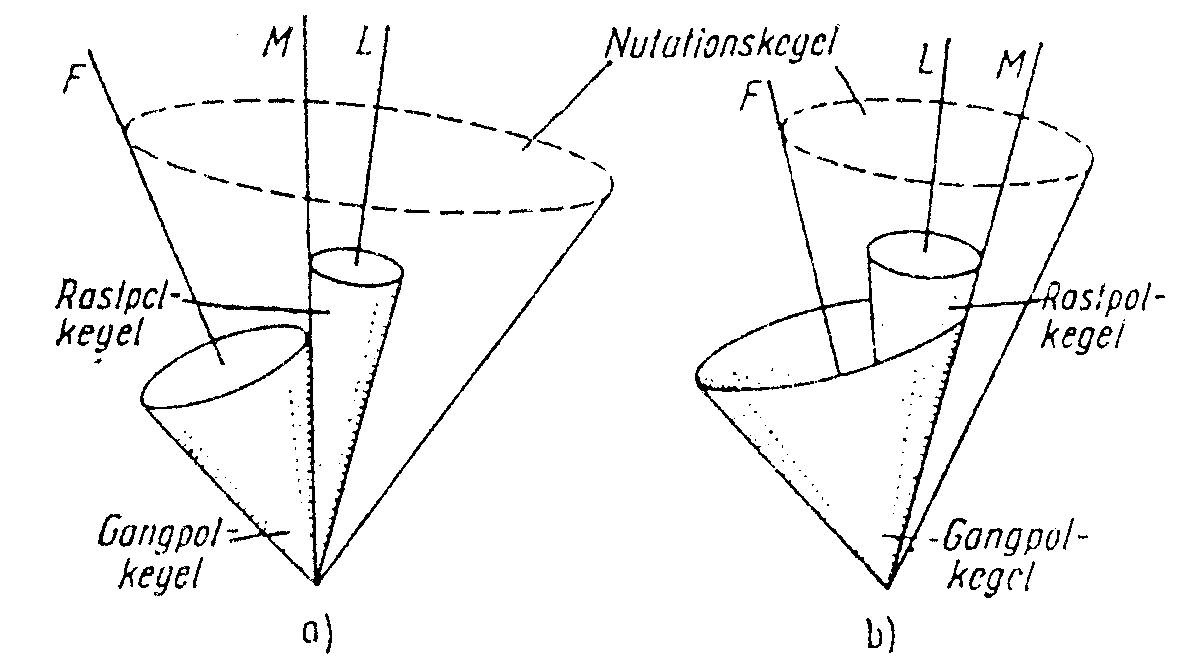
\includegraphics[width=0.7\textwidth]{nutationskegel.png}
    \caption{Nutationsbewegung eines Kreisel \citep[vgl.][]{Uni_aachen}}
\end{figure}\\
Im Fall a) spricht man von einem verlängerten Kreisel, da die Figurenachte die Hauptträgheitsachse mit dem kleinsten Trägheitsmoment ist.\\
Im Fall b) spricht man von einem abgeplatteten Kreisel, da die Figurenachte die Hauptträgheitsachse mit dem größten Trägheitsmoment ist. \citep[vgl.][]{Uni_aachen}\\%\footnote{\url{https://web.physik.rwth-aachen.de/~fluegge/Vorlesung/PhysIpub/Exscript/6Kapitel/VI12Kapitel.html}}
Die Rotation kommt dadurch zustande, dass der Raspolkegel den Gangpolkegel abrollt.
Der Nutationskegel beschreibt die so entstandene Bewegung, der Rotationsachse um den ortsfesten Drehimpuls.
\section{Präzessionsfrequenz und Präzessionsrichtung des Kreisels}\label{sec:Praezession}
\textbf{Zeigen Sie, dass die Präzessionsfrequenz durch Gl. (12) gegeben ist! Wie hängt diese vom Winkel zwischen der Figurenachse und der Horizontalen ab? Wie hängt die Präzessionsrichtung von der Drehrichtung des Kreisels ab?}\\
Ein Kreisel, welcher um den Winkel $\alpha$ zu seiner Figurenachse gedreht ist,
übt folgendes Drehmoment aus:
\begin{align}
    M&=m\cdot g\cdot r\cdot\sin(\alpha)
\end{align}
Der präzendirende Kreisel, dessen Drehimpuls und Rotationsachse nicht zusammen fallen, übt auch ein Drehmoment aus.
\begin{align}
    \vec{M}&=\vec{\omega}_\text{P}\times\vec{L}\\
    M&=\omega_\text{P}\cdot L \cdot\sin(\alpha)
\end{align}
Durch Gleichsetzen erhält man:
\begin{align}
    M&=\omega_\text{P}\cdot L \cdot\sin(\alpha)\\
    m\cdot g\cdot r\cdot\sin(\alpha)&=\omega_P\cdot L \cdot\sin(\alpha)\\
    \omega_\text{P}&=\frac{m\cdot g\cdot r}{L}
\end{align}
Da sich der Kreisel um die Achse mit dem kleinsten Trägheitsmoment dreht, folgt für den Drehimpuls: \(L=J_3\cdot\omega_3\).
Somit folgt für die Präzessionsfrequenz:
\begin{align}
    \omega_\text{P}&=\frac{m\cdot g\cdot r}{L}\\
    &=\frac{m\cdot g\cdot r}{J_3\cdot\omega_3}
\end{align}
\section{Funktionsprinzip eines Kreiselkompasses}
\textbf{Beschreiben Sie das Funktionsprinzip eines Kreiselkompasses!}\\
Ein Kreiselkompass besteht aus einem schnell drehenden Kreisel,
welcher an einer Kardanischen Aufhängung aufgehangen wird.
An einer Kardanischen Aufhängung kann sich der Kreisel um jede Achse frei drehen.
Sein Drehimpuls zeigt nach Norden.
Es wird ein Drehmoment erzeugt, wenn dieser nun nicht mehr nach Norden zeigt.
Dieser versucht jedoch sich wieder nach Norden auszurichten um die Drehimpulserhaltung nicht zu verletzen.\\
Ein Kreiselkompasses hat den entscheidenden Vorteil zu einem konventionellen Kompass, dass dieser unabhängig von Erdmagnetfeld ist.
\section{Bierfilz-Wurf}
\textbf{Wirft man einen Bierfilz schräg nach oben, und gibt ihm gleichzeitig eine Drehung um seine Figurenachse wie einem Diskus, so richtet er sich senkrecht auf (Probieren Sie es ruhig aus!). Warum? In welche Richtung geschieht das Aufrichten und wie rotiert der senkrecht stehende Bierfilz? Warum passiert dies nicht beim Diskus?}\\
Wirft man ein Bierfilz oder Spielkarte schräg nach oben, während sich dieses um seine Figurenachse dreht, richtet sich seine Figurenachse horizontal aus.
Hierbei ist es egal, wie schräg es nach oben gewurfen wurde, es ist immer das gleiche zu beobachten.
Bei einer stärkteren Drehung um seine eigene Achse tritt das Ergebnis schneller ein.\\
Die Beobachtung kann erklärt werden, dass sowohl durch den Luftwiderstand als auch die Gravitation eine Kraft auf den Bierfilz wirkt.
Diese Kraft bewirkt ein Drehmoment, welches der Filz kippt.
Somit "kippt" der Filz in die Horizontale, damit die angreifenden Kräft minimal werden (Gravitationskraft parallel zum Drehimpuls).\\
Der Diskus ist so konzipert, dass einen sehr großen Abstand zum Mittelpunkt hat.
Dies führt zu einen sehr großen Trägheitsmoment.
Somit reichen die angreifenden Kräft nicht aus ein so großes Drehmoment zu erzeugen.
Dieser würde eher auf dem Boden ankommen bevor er in die Horizontale kippt.

